\section{Project Overview}
\subsection{Toolbox}
I implemented my whole project on Windows, using Visual Studio Community 2017. And I used some open-source libraries: Eigen \cite{eigenweb}, Libigl \cite{libigl}, LBFGS++\cite{LBFGSpp}, and OpenMesh \cite{Botsch02openmesh}. The needed libraries are compiled into static libraries file (*.lib), and included in the projects.

\subsubsection{OpenMesh}
OpenMesh \cite{Botsch02openmesh} is the core data sturcture of my project. This library implements so-called halfedge data structure for polygonal mesh.

Each mesh $M = (V, E, F, H)$ can be represented by four components: $V$ stands for vertex set, $E$ stands for edge set, $H$ stands for halfedge setsand $F$ stands for face set. Each edge is corresponded with two opposite halfedges. The linking relations are shown in Fig.\ref{fig:halfedge}.

\begin{figure}
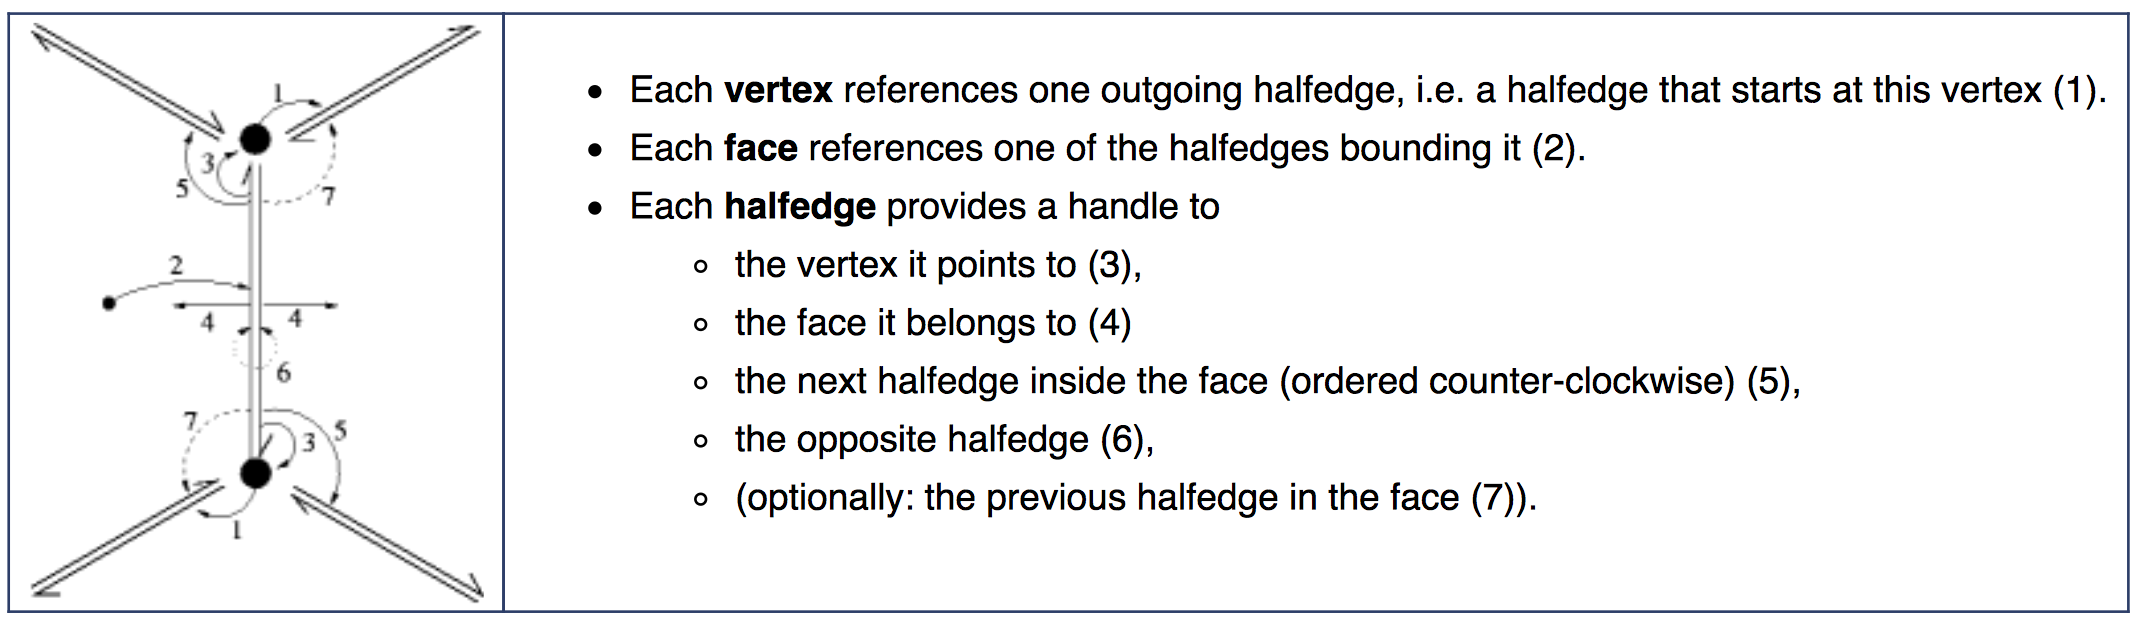
\includegraphics[width=0.9\textwidth]{images/halfedge}
\caption{Halfedge data structure.}
\label{fig:halfedge}
\end{figure}

\subsubsection{Eigen}
Eigen \cite{eigenweb} is a standard library to handle matrices and their operations in C++. It's a head-only library, so it's very easy to deploy.

I will use this library to handle linear part in my project.

\subsubsection{LBFGS++}
LBFGS is a first-order optimization algorithm with line search. LBFGS++ \cite{LBFGSpp} is an implementation for this algorithm in C++. This is a project I found on GitHub, and it is very new. 

I use this algorithm to optimize the energy for hyperbolic orbifold.

\subsubsection{Libigl} 
Libigl \cite{libigl} is a simple C++ geometry processing library. 

I use the Viewer class \footnote{\url{http://libigl.github.io/libigl/tutorial/tutorial.html\#viewermenu}} of this library to implement my GUI. The GUI part of this library is based on Nanogui\footnote{\url{https://github.com/wjakob/nanogui}} and OpenGL3. The GUI of my project is shown in Fig.\ref{fig:GUI}

\begin{figure}
\centering
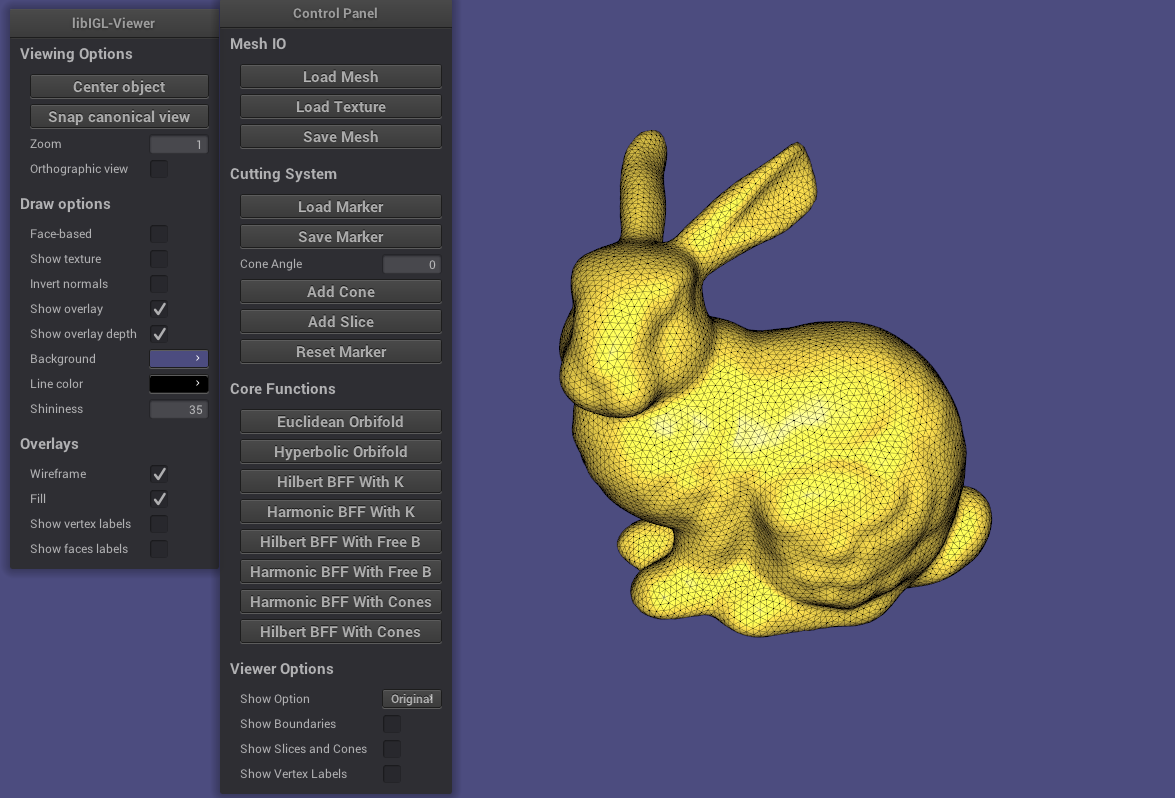
\includegraphics[width=0.7\textwidth]{images/gui}
\caption{The GUI of my project}
\label{fig:GUI}
\end{figure}


On the other hand, this library provides lots of functions used in geometry processing. I also use its quadratic programming algorithm \footnote{\url{http://libigl.github.io/libigl/tutorial/tutorial.html\#quadraticprogramming}}. It is used in the optimization problem for closed loop in boundary first flatten algorithm.

\subsection{Project Structure}
I put all codes in one solution of VS2017. The solution have five VS projects: Mesh, OrbifoldEmbedding, BoundaryFirstFlattening, Viewer and Utilities. They are linked together by reference between static libraries.

\textbf{Mesh}
In this VS project, I extend the default definitions of OpenMesh. This mesh structure are used in all of other subprojects.

\textbf{OrbifoldEmbedding} 
This VS project implements the algorithms in \cite{Aigerman:2015:OTE:2816795.2818099}\cite{Aigerman:2016:HOT:2980179.2982412}. Both Euclidean orbifold Tutte embedding and hyperbolic orbifold Tutte embedding are included in this project.

\textbf{BoundaryFirstFlattening}
This VS project implements the algorithms in \cite{1704.06873}.

\textbf{Viewer}
This VS project implements the GUI part of my project. Meshes, embedding results, and texture mappings are showned here.
Besides, I extend the Viewer class of Libigl so that I can select vertices on a mesh interactively.

\textbf{Utilities}
This VS project implements some auxiliary functions needed in my project.
The core function for my project is MeshSlicer, used to cut the mesh into a disk. This operation is needed for both orbifold and BFF algorithms. But most of this code is from my previous research projects. I modify it so that I can interactively choose slices.
Most of other functions here are used to show my results.







